% Copyright Aidan Randle-Conde 2007-2014
% http://www.aidansean.com/phd_notes
% Anyone is free to download, redistribute, edit and use these notes and the source tex files with the following restrictions:
% This 
%  This message is included in the tex source files.
%  Aidan Randle-Conde is credited as the author.
%  Images are correctly credited to their respective authors, as outlined in the references.
%  No part of these notes may be used for commercial purposes.

\chapter[Matter and forces]{Matter and forces}
\chaptermark{Matter and forces}

\section{Leptons}

\[
  \begin{array}{ccccccc}
    \begin{array}{c}
    Charge = 0 \\
    Charge = 1
    \end{array}
    
  \left(
    \begin{array}{c}
    \nu_e \\
    e
    \end{array}
  \right)
  
    \begin{array}{c}
    \\
    0.5 \mev
    \end{array}
  
  \left(
    \begin{array}{c}
    \nu_{\mu} \\
    \mu
    \end{array}
  \right)
  
    \begin{array}{c}
    \\
    0.1 \gev
    \end{array}
  
  \left(
    \begin{array}{c}
    \nu_{\tau} \\
    \tau
    \end{array}
  \right)
  
    \begin{array}{c}
    \\
    1.8 \gev
    \end{array}
  \end{array}
\]

Leptons do not experience the strong force but do experience the electromagnetic and weak forces.

\section{Quarks}

\[
  \begin{array}{ccccccc}
    \begin{array}{c}
    Charge =  2/3 \\
    Charge = -1/3
    \end{array}
    
  \left(
    \begin{array}{c}
    u \\
    d
    \end{array}
  \right)
  
    \begin{array}{c}
    0.3 \gev \\
    0.3 \gev
    \end{array}
  
  \left(
    \begin{array}{c}
    c \\
    s 
    \end{array}
  \right)
  
    \begin{array}{c}
    1.5 \gev \\
    0.5 \gev
    \end{array}
  
  \left(
    \begin{array}{c}
    t \\
    b
    \end{array}
  \right)
  
    \begin{array}{c}
    180 \gev \\
    5 \gev
    \end{array}
  \end{array}
\]

The $u$, $d$, $s$ are ``constitutional'' masses which one can infer from the masses of the corresponding hadronic systems.  However it is thought that most if this mass is "effective" ie generated dynamically by the strong interaction.  Intrinsic masses are $\sim 4\mev (u,d)$ and $100\mev(s)$.

\begin{itemize}
  \item We do not understand the masses of the particles
  \item They are all fermions (spin$-1/2$)
  \item The $u$ and $d$ quarks combine to form the hadorns we know
  \item The above is believed to constitute about 4\% of the mass-energy of the universe
\end{itemize}

Forces are mediated by bosons (integer spin) and can be thought to arise from local gauge invariance.

\section{Gravity}

This is by far the weakest force and is thought to be mediated by spin$-2$ gravitons.

It is important on an astronomical scale because of the large masses multiplying the intrinsic weakness of the force.  Gravity is universal and there are no cancellations (ie no negative causes).

Gravitational radiation should arise when masses oscillate, giving quadrupole radiation.  Gravitational radiation would create a ripple in space-time.  Indirect detections exist from observations by Hulse and Taylor over a seventeen year period of a binary system of two neutron stars.  The change in the period of the binary system can only be accounted for by the emission of gravitational radiation, winning the Nobel Prize in 1993.

\subsection{The Planck mass}

Suppose two pointlike masses $m$ are created by quantum fluctuations out of the vacuum.  One mass can exist for a time $\delta t$ given by:

\begin{eqnarray*}
  \delta \epsilon \delta t & \le & \hbar \\
  mc^2 \delta t & \sim & \hbar \\
  \Rightarrow \delta t & \sim & \frac{\hbar}{mc^2} \\
  \textrm{Range } r & = & c \delta t \\
  & = & \frac{\hbar}{mc}
\end{eqnarray*}

At this separation the gravitational potential $V_G$ is given by:

\begin{eqnarray*}
  V_g & = & \frac{Gm^2}{r} \\
  & = & \frac{Gm^3c}{\hbar}
\end{eqnarray*}

If $V_G$ becomes comparable with the energy $mc^2$ the relativistic effects become important, but there is no theory of quantum gravity.

\begin{eqnarray*}
  \textrm{So } \frac{Gm^3c}{\hbar}\frac{1}{mc^2} & \sim & 1 \\
  \textrm{So } m_{Planck} & \simeq & \sqrt{\frac{\hbar c}{G}} \\
  &\simeq & 10^{19} \\gev
\end{eqnarray*}

Similarly:

\begin{eqnarray*}
  \textrm{Planck length: } & & 2 \times 10^{-35}\units{m} \\
  \textrm{Planck time:}    & & 10^{-44} \units{s}
\end{eqnarray*}

Without quantum gravity we cannot discuss the evolution of the universe at epochs around and before the Planck time.

\subsection{Dark matter}

Dark matter is believed to constitute about 25\% of the matter-energy content of the universe.  This comes from evidence from velocity rotation curves in a galaxy, as shown in figure \ref{fig:ch1_galacticCurve}.

\begin{figure}[!htb]
  \begin{center}
    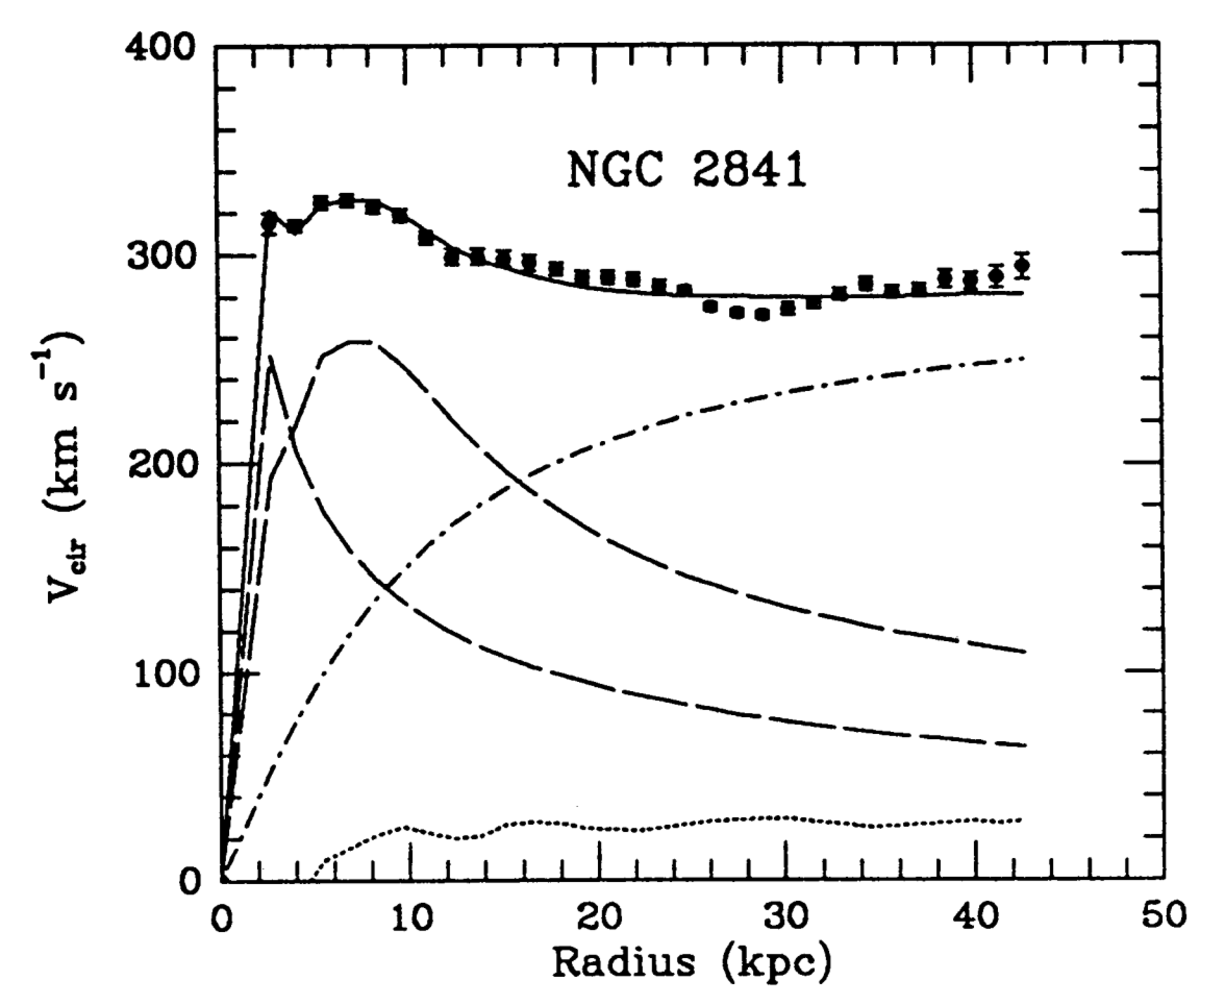
\includegraphics[width=\textwidth]{images/chapter_1/galacticCurve.pdf}
    \caption[Rotational curve of NGC 2841]{Rotational curve of NGC 2841  Predictions are shown for visible matter (dashed line), gas (dotted line), dark matter halo (dash-dot line) and total (solid line).  Data points show measurements. \cite{galacticCurve}}
    \label{fig:ch1_galacticCurve}
  \end{center}
\end{figure}

The radial velocity of a star is measured using the doppler shift and is plotted as a function of the distance from the centre of the galaxy, $r$.

\begin{eqnarray*}
  \textrm{Centripetal force} & = & \textrm{Gravitational force} \\
  \textrm{For } r<R : && \\
  \frac{\Delta m v^2(r)}{r} & = & \frac{G \Delta m M_{r<R}}{r^2} \\
  v^2(r) & = & \frac{GM_{r<R}}{r} \\
  & = & \frac{G}{r}M_s \left( \frac{r}{R} \right)^2 \\
  & = & \frac{GM_sr^2}{R^3} \\
  \textrm{So } v(r) & \propto & r \textrm{ for } r<R \\
  \textrm{For } r>R: && \\
  \frac{\Delta m v^2(r)}{r} & = & \frac{GM_s \Delta m}{r} \\
  v^2(2) & = & \frac{GM_s}{r} \\
  \textrm{So } v(r) & \propto & \frac{1}{\sqrt{r}} \textrm{ for } r>R
\end{eqnarray*}

\begin{figure}[!htb]
  \begin{center}
    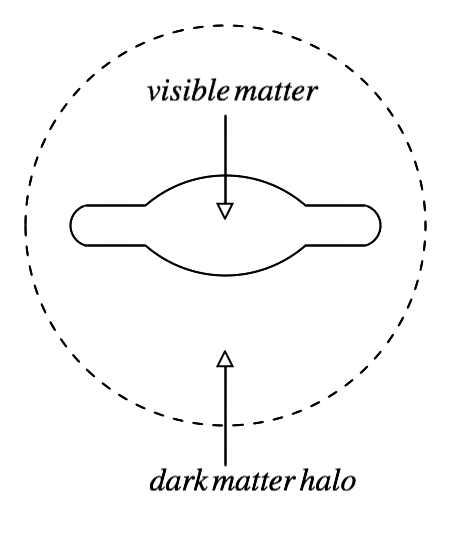
\includegraphics[width=0.5\textwidth]{images/web_feynman/image_88.png}
    \caption[Dark matter halo around a galaxy]{Dark matter halo around a galaxy.}
    \label{fig:ch1_darkMatterHalo}
  \end{center}
\end{figure}

The observed discrepency is hypothesised to be the result of dark matter.  It is thought that there is a halo of dark matter surrounding the galaxy with a matter distribution which yields the observed discrepency.

\subsection{Candidates for dark matter}

\begin{description}
  \item[Neutrinos]There is now evidence that neutrinos have mass.  However the masses are small and neutrinos are therefore relativistic particles, so this is hot dark matter which does not stay around long enough to provide gravitational binding.
  \item[Brown dwarves (Massive cool hadronic objects - MaCHOs)]Brown dwarves are like small stars which are not massive enough for nuclear burning so they appear dark.  There cannot be too many brown dwarves since there would then be too much baryonic matter which is incompatible with current understanding of the abundance of hydrogen, helium and deuterium in the early universe.  The elements were generated in the first $\simeq 900 s$.  To search for brown dwarves it is necessary to look at many stars in eg a large Magellic cloud.  If a brown dwarf passes across the line of sight of one of the stars then through gravitational lensing the light intensity from the star will increase and decrease in a characteristic way.  Brown dwarves have been observed but not in sufficient numbers to account for the amount of dark matter.
  \item[Supersymmetric particles]There are several names for such particles.  In the context of dark matter a common name is Weakly Interacting Massive Particles (WIMPs).  Alternatives include Lightest Symmetrical Particles (LSPs) and candidates thereof (neutralinos, gravitinos etc).
\end{description}

The current standard model of cosmology gives 5\% of the matter observed, 25\% dark matter and 70\% dark energy.  Where does this sub-division come from?

A survey of Type I supernovae (see figure \ref{fig:ch1_type1Supernovae}) indicates that the universe is accelerating for $z \ge 0.8 (z = \delta \lambda/\lambda)$.  The type I supernovae are like ``standard candles'' in a binary system in which matter flows from one of the stars to another and creates a thermonuclear explosion.  This constitutes the standard candle and therefore the distance can be determined.  The doppler shift gives the recessional velocity.

\begin{figure}[!htb]
  \begin{center}
    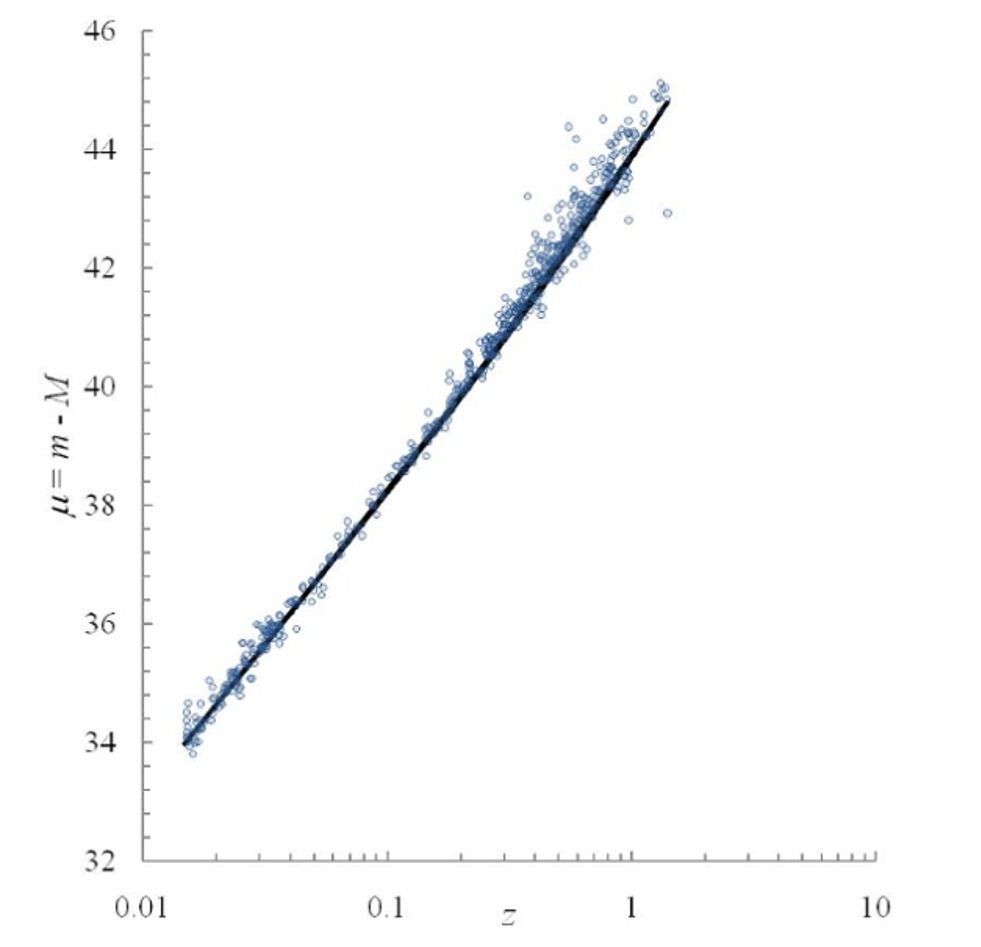
\includegraphics[width=0.5\textwidth]{images/chapter_1/type1Supernovae.pdf}
    \caption[Survey of type I supernovae]{Survey of type I supernovae. \cite{typeOneSupernovae}}
    \label{fig:ch1_type1Supernovae}
  \end{center}
\end{figure}

\subsection{Anisotropies in the cosmic microwave background and the history of the universe}

The universe is now thought to be $\sim 14 \times 10^9$ years old.  After about $350,000$ years the temperature had dropped to about $3000K$, at which point electrons and protons could combine to form hydrogen.  At this epoch, photons decoupled from matter.  Subsequently this black body spectrum cooled to $2.7K$, which is what is observed today.  This was first observed in 1965 by Perzies and Wilson, receiving the Nobel Prize in 1978.  The cosmic microwave background radiation is uniform tp $1$ part in $10^5$ in all directions.

Big bang nucleosynthesis occured in the first $900s$.  Electroweak symmetry breaking took place at $10^{-12}s$ or $E\sim 100\gev$.  The energy released by this symmetry breaking drives cosmic inflation which explains the flatness of the universe and the horizon problem.  Grand unified theory symmetry breaking occues at $10^{15} \gev$.

Anisotropies were originally measured by the COBE sattelite and by other experiments, most recently Planck (as shown in figure \ref{fig:ch1_powerSpectrum}), WMAP and Boomerang.

\begin{figure}[!htb]
  \begin{center}
    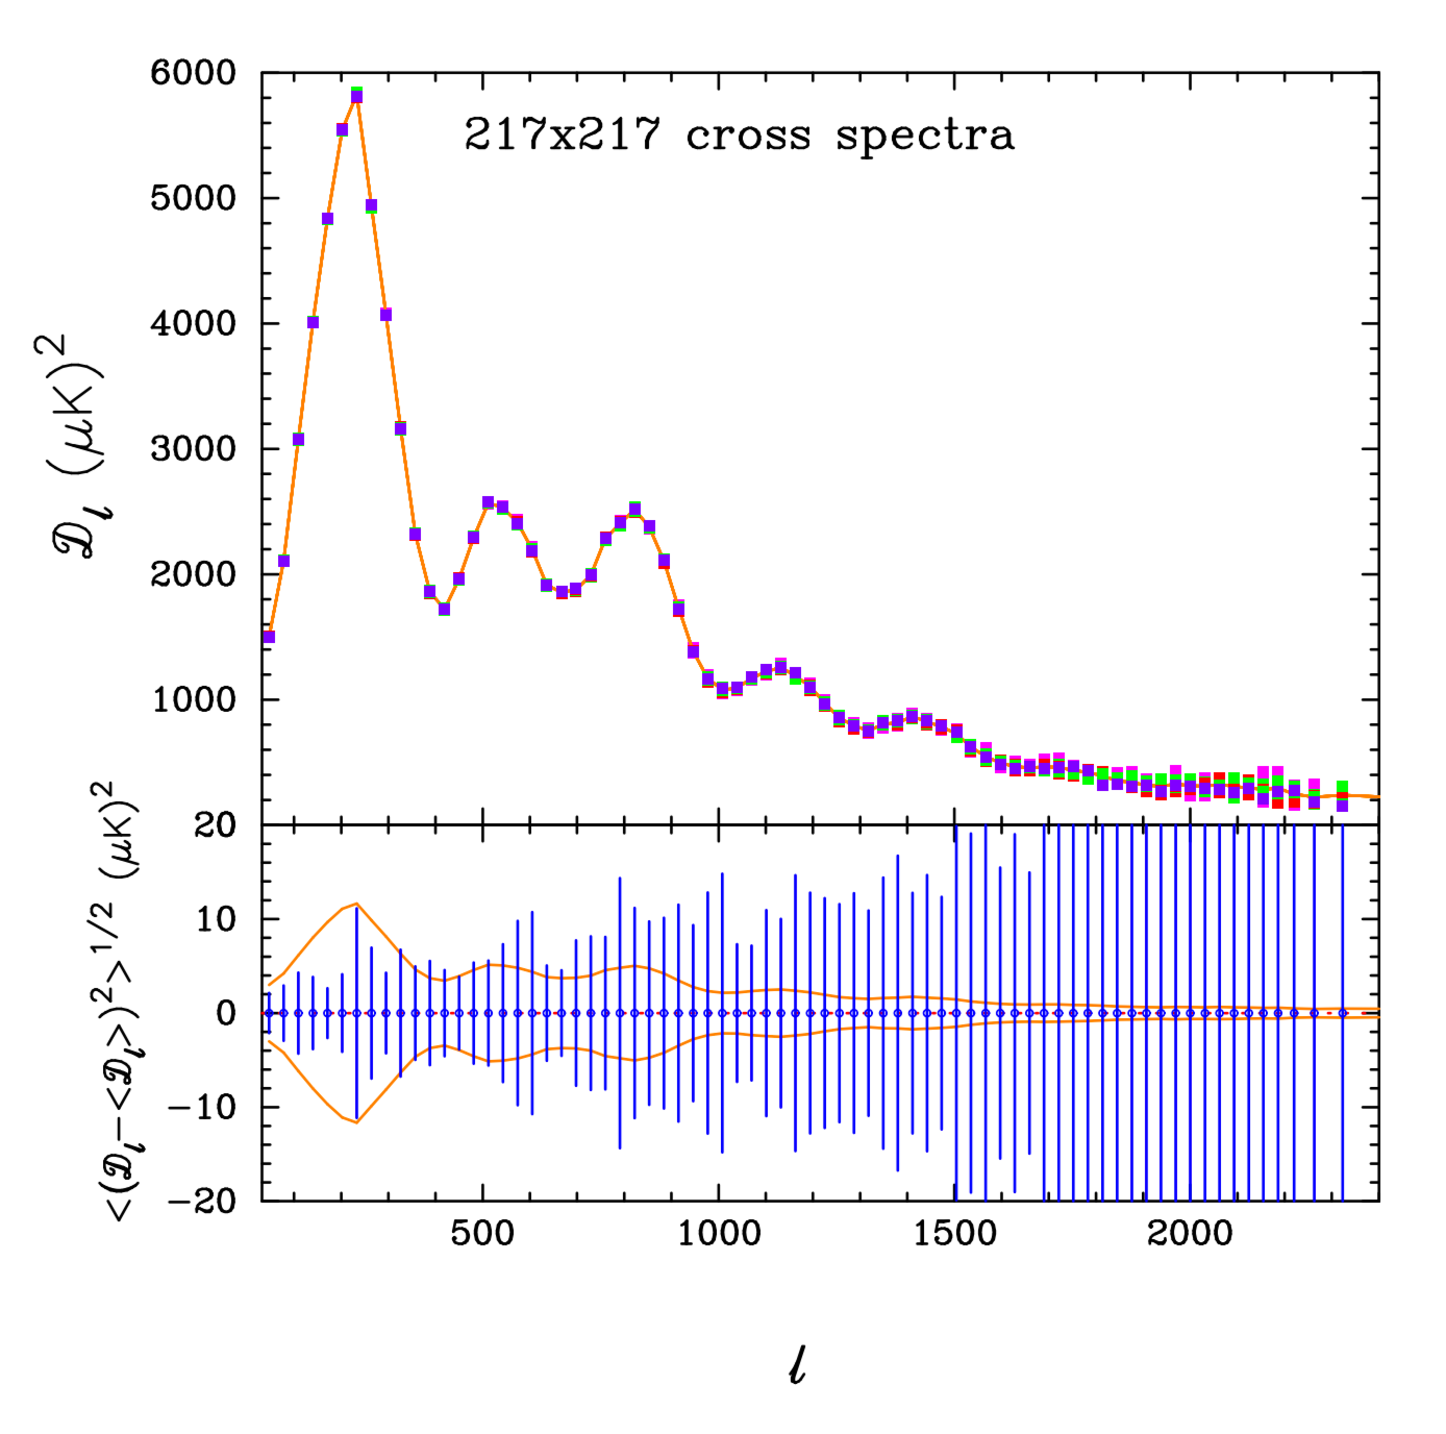
\includegraphics[width=\textwidth]{images/chapter_1/powerSpectrum.pdf}
    \caption[Cross spectra ``power spectrum'' plot (Planck)]{Cross spectra ``power spectrum'' plot (Planck). \cite{powerSpectrum}}
    \label{fig:ch1_powerSpectrum}
  \end{center}
\end{figure}

The power spectrum gives strong evidence for:
\begin{itemize}
  \item a flat universe
  \item inflation
  \item ratio of dark energy : dark matter of 70\% : 25\%
\end{itemize}

\section{The weak force}

The weak force is mediated by massive vector bosons:

\begin{eqnarray*}
  W^{\pm} & M_W & \sim 80.4 \gev \\
  Z^0     & M_Z & \sim 91.2 \gev
\end{eqnarray*}

The instrinsic strength of the force, $g_W$, is of the same order as the electromagnetic force, but the massive force carriers make it appear weak and short ranged.

For electromagnetism the strength is $\e^2/q^2$, where $q$ is the propagator momentum.  For the weak force the strength is $g^2_W/(q^2 + M^2_W)$.  Some examples of weak interactions include:

\begin{eqnarray*}
  n                   & \to & p \quad \e^- \quad \bar{\nu}_e \\
  \nu_e \quad n       & \to & p \quad \e^- \\
  \bar{\nu}_e \quad p & \to & n \quad \e^+ \\
  \bar{\nu}_e \quad u & \to & d \quad \e^+
\end{eqnarray*}

Figure \ref{fig:ch1_NToPENu} shows the Feynman diagram for a weak scattering process.

\begin{figure}[!htb]
  \begin{center}
    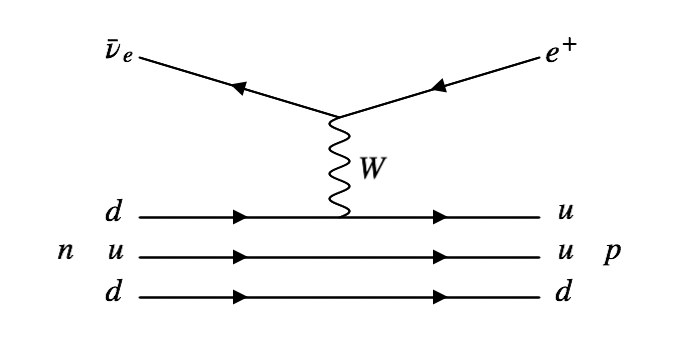
\includegraphics[width=0.8\textwidth]{images/web_feynman/image_1.png}
    \caption[Feynman diagram of proton-antineutrino scattering]{Feynman diagram showing the process $\bar{\nu}_e p \to e^+ n$.}
    \label{fig:ch1_NToPENu}
  \end{center}
\end{figure}

Some pure leptonic weak processes is shown in figures \ref{fig:ch1_NueEToNumMu} and \ref{fig:ch1_ENueToENue}.

\begin{figure}[!htb]
  \begin{center}
    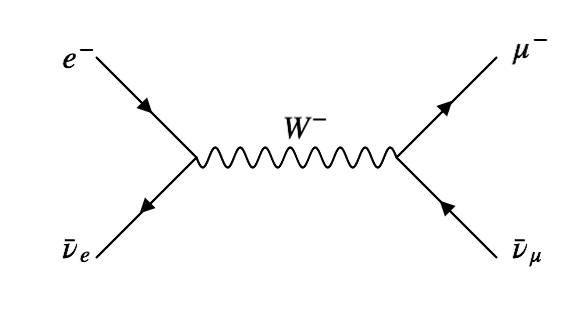
\includegraphics[width=0.8\textwidth]{images/web_feynman/image_2.png}
    \caption[Feynman diagram of lepton scattering]{Feynman diagram showing the process $\bar{\nu}_e e^- \to \bar{\nu}_\mu \mu^-$.}
    \label{fig:ch1_NueEToNumMu}
  \end{center}
\end{figure}

\begin{figure}[!htb]
  \begin{center}
    \begin{tabular}{cc}
      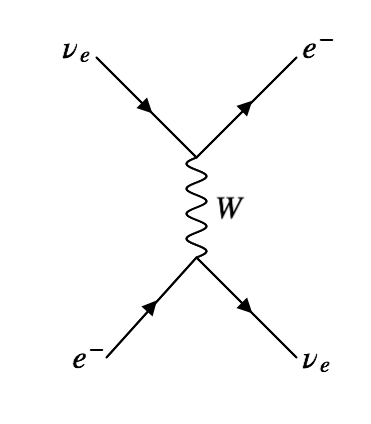
\includegraphics[width=0.4\textwidth]{images/web_feynman/image_3.png} &
      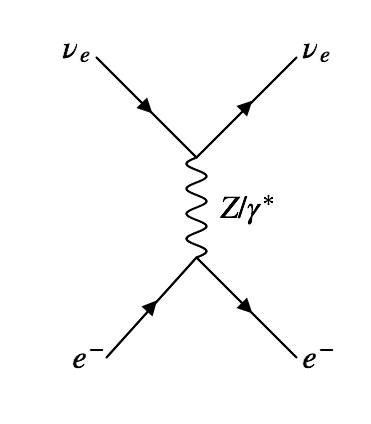
\includegraphics[width=0.4\textwidth]{images/web_feynman/image_4.png}
    \end{tabular}
    \caption[Feynman diagram of lepton scattering]{Feynman diagram showing the elastic scattering process $\nu_e e^- \to \nu_e e^-$.}
    \label{fig:ch1_ENueToENue}
  \end{center}
\end{figure}

\clearpage

\section{The electromagnetic interaction (QED)}

The electromagnetic force is mediated by the massless photon, which has an infinite range.  The coupling constant, $e$, is quantised $(0,\pm 1/3,\pm 2/3,\pm 1)$ and is not too strong, so perturbation theory works.

The strength of the force is characterised by $\alpha$:

\[
  \alpha = \frac{\e^2}{\hbar c} = \frac{\e^2_{Coulomb}}{4\pi \epsilon_0 \hbar c} = \frac{\e^2_{HL}}{4 \pi \hbar c}
\]

where $e_{Coulomb}$ is the Coulomb charge and $e_{HL}$ is the Heaviside-Lorentz charge.

In particle physics $e$ is measured in Heaviside-Lorentz units where $\hbar = c = 1$.

\[
  \textrm{Therefore } \alpha = \frac{\e^2}{4\pi} \simeq \frac{1}{137.04}
\]

\subsection{The physical meaning of \texorpdfstring{$\alpha$}{Alpha}}

$\alpha$ expresses the energy of an $\e^+ \e^- $ pair materialising for a short time in the vacuum as a fraction of the rest mass energy $m_e c^2$:

\begin{eqnarray*}
  \alpha & \sim & \frac{\e^2}{c \Delta t}\frac{1}{m_e c^2} \\
  \Delta t \Delta E & \sim & \hbar \\
  \Delta t & \sim & \frac{\hbar}{m_e c^2} \\
  \textrm{So } \alpha & \sim & \frac{\e^2}{c}\frac{m_e c^2}{\hbar}\frac{1}{m_e c^2} \\
  & = & \frac{\e^2}{\hbar c}
\end{eqnarray*}

\section{The strong force (QCD)}

Since the 1950s, it was knwon that the $\Delta^{++}(uuu)$ particle state existed at $1238 MeV$, formed in $\pi^+ p$ scattering:

\[
  \pi^+ \quad p \stackrel{\Delta^{++}}{\to} \pi^+ \quad p
\]

In the simple quark model there are 3 up quarks, each with psin$-1/2$ in the same direction.  Also in 1965 the $\Omega^-$ was discovered which consists of 3 strange quarks each with spin$-1/2$ in the same direction.  These appeared to violate the Pauli exclusion principle.

The solution was introduce 3 colour charges with the strong force mediated by massless gluons which carry colour.  The force is not of infinite rane because the strength increases with separation, leading to confinement.

\section{Local gauge invariance}

The weak, electromagnetic and strong forces all appear to arise from requiring local gauge invariance.  This means that the Lagrangians are invariant with respect to a local gauge transformation and equations of motion derived from the Lagrangian are invariant with respect to local gauge transformation.

Quantum states can be multiplied by a phase factor:

\[
  \psi'(x,t) \to \e^{iq \chi(x)}\psi(x,t)
\]

If $\chi(x,t)$ depends on space and time then the above expression is a local gauge transformation.  To allow this the electromagnetic field, $A_{\mu}$ must transform in a specific way.

In weak interactions this is not as simple.  The Lagrangian contains four massless bosons ($W^i,B$).  To allow for local gauge invariance, weak isospin and weak hypercharge matrices are required which combine with the massless vector fields to form the gauge transformation.  Symmetry breaking occurs such that $W^1_{\mu}$ and $W^2_{\mu}$ yield $W^{\pm}$ and $W^3_{\mu}$ and $B_{\mu}$ mix to yield $A_{\mu}$ and $Z^0$.  This then unifies the electromagnetic and weak interactions via the Higgs mechanism.

\section{Grand unification (GUTs)}

The GUT attemps to unify the electromagnetic, weak and strong forces.  The coupling constants evolve with energy due to loop processes, as indicated in figure \ref{fig:ch1_runningCoupling}.

\begin{figure}[!htb]
  \begin{center}
    \begin{tabular}{ccc}
      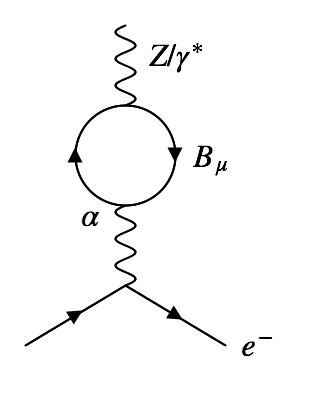
\includegraphics[width=0.3\textwidth]{images/web_feynman/image_5.png}
      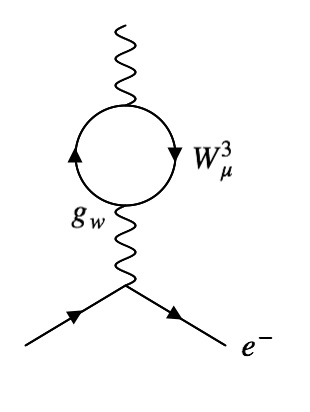
\includegraphics[width=0.3\textwidth]{images/web_feynman/image_6.png}
      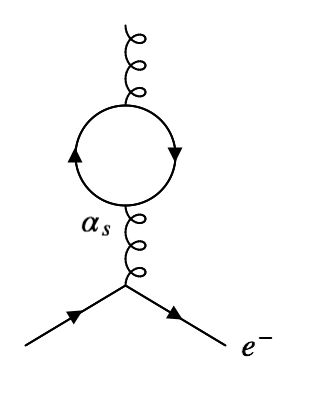
\includegraphics[width=0.3\textwidth]{images/web_feynman/image_7.png}
    \end{tabular}
    \caption[Loop processes affecting running couplings]{Typical loop processes affecting running couplings for the electromagnetic (left), weak (centre), and strong (right) processes.}
    \label{fig:ch1_runningCoupling}
  \end{center}
\end{figure}

The couplings are expected to merge at $\sim 10^{15}\gev$ according to some models, but the couplings do not come together at this energy.  The evolution of $g_1$, $g_2$, $g_3$ could coincide if supersymmetric particles exist, as shown in figure \ref{fig:ch1_SUSYUnification}.  This would then yield a grand unified group, $G$, or $SU(5)$ which is a combination of the three groups describing the three forces.  Here gauge bosons exist which would allow quarks to turn into leptons.  This would also allow protons to decay:

\[
  p \to \e^+ \quad \pi^0
\]

This decay has been extensively searched for but not observed.  This places a lower limit on the lifetime of the proton at $\tau_p > 10^{30}$ years.

\begin{figure}[!htb]
  \begin{center}
    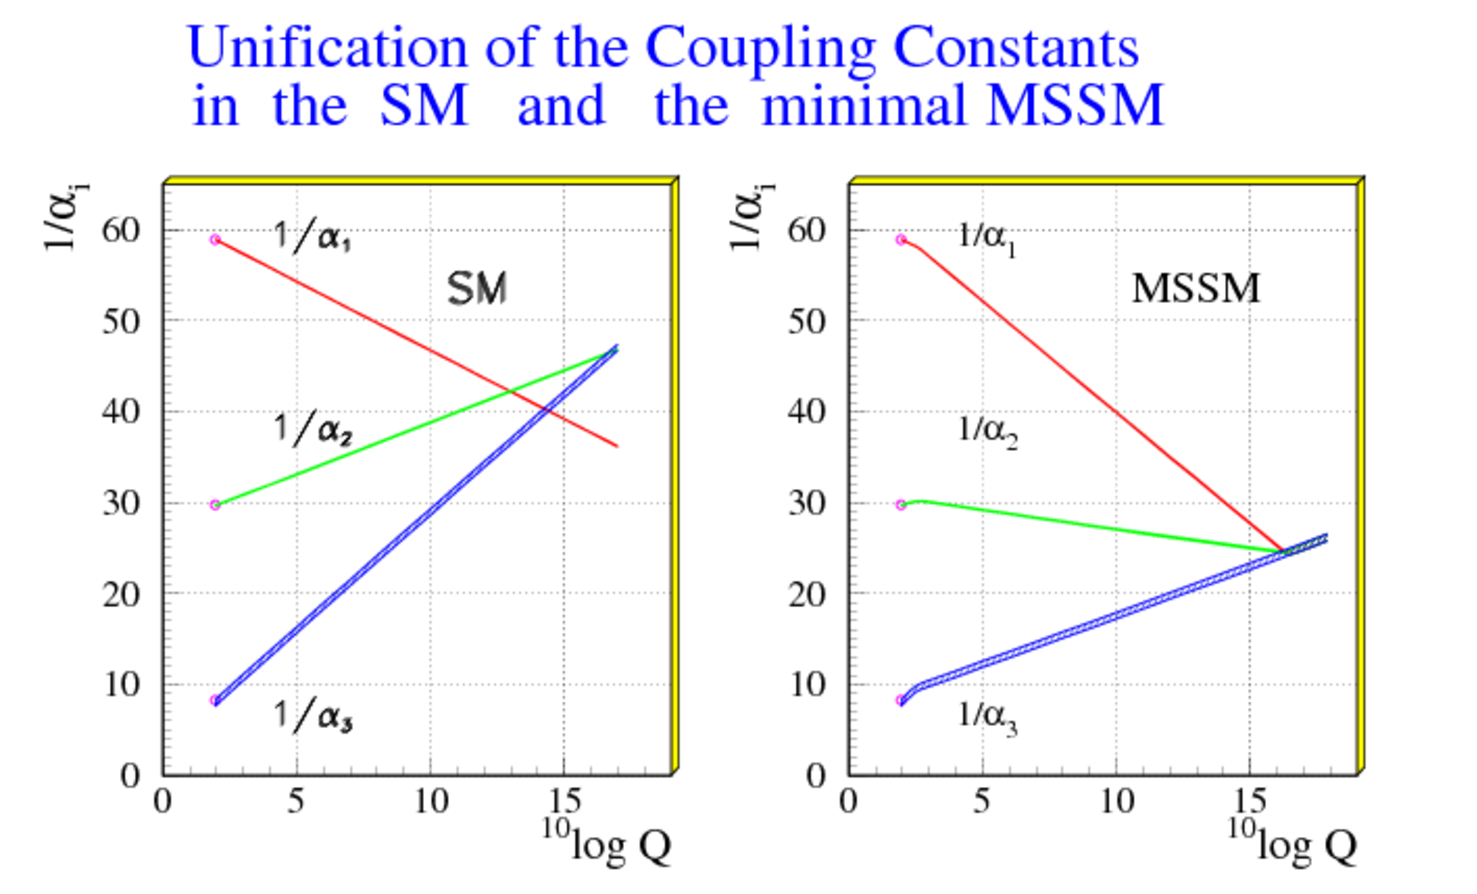
\includegraphics[width=\textwidth]{images/chapter_1/SUSYUnification.pdf}
    \caption[Running couplings and unification]{Running couplings and unification over a wide range of energies for the Standard Model (left) and with supersymmetric models (right). \cite{SUSYUnification}}
    \label{fig:ch1_SUSYUnification}
  \end{center}
\end{figure}
